\section{Dense Iterative Solvers}
\label{sec:iterative_solvers}

The goal of an iterative method is to generate a sequence of increasingly accurate approximate solutions $\hat{x}$ for a linear system $Ax=b$. In such a framework, the main goal it to replace the dense matrix $A$ by a matrix $M$ that is easier to solve (i.e. has a reduced complexity). This can either be achieved by a reduced size, or special characteristics that allow for solving in $\mathcal{O}(n^2)$ or $\mathcal{O}(n)$. Therefore, as long as a desired accuracy can be achieved by a short sequence of approximate solutions, iterative methods can be considerably faster than direct ones, which require $\mathcal{O}(n^3)$. Depending on the general idea behind how this matrix $M$ is created, several different iterative methods can be distinguished. A summary of those approaches together with the most popular methods for each of them, will be provided in the following sections.

\import{2_3_iterative_solvers}{2_3_1_stationary_methods.tex}
\import{2_3_iterative_solvers}{2_3_2_subspace_methods.tex}
\import{2_3_iterative_solvers}{2_3_3_krylov_methods.tex}

\newpage


%OLD
The goal of an iterative method is to generate a sequence of increasingly accurate approximate solutions $\hat{x}$ for a linear system $Ax=b$. In such a framework, the matrix $A$ is typically only involved in terms of matrix-vector multiplications, which can be calculated in order of $\mathcal{O}(n^2)$ for a dense matrix \cite{golub_matrix_2013}. Therefore, as long as a desired accuracy can be achieved by a short sequence of approximate solutions, iterative methods are considerably faster than direct solvers (which require $\mathcal{O}(n^3)$). Such techniques are especially common in the context of sparse matrices, where the calculation of the matrix vector product can achieved in (almost) linear complexity.

Many classical iterative methods, such as Jacobi or Gauss-Seidel (see \cite{golub_matrix_2013} or \cite{saad_iterative_2003}) are based on a \textit{splitting} of the original matrix $A$:
\begin{equation}
\label{eqn:splitting}
    A = M - N
\end{equation}

\noindent and thus the iterative solutions can be created by:
\begin{equation}
    Mx^k = Nx^{k-1} +b = (M-A)x^{k-1}+b
\end{equation}

\noindent While this might just look like a regularization of the original problem, the trick to achieving a reduced complexity is in how to choose the splitting in Equation~\hyperref[eqn:splitting]{\ref{eqn:splitting}}. The matrix $M$ has to be chosen in such a way, that its characteristics (for example diagonal structure in Jacobi and lower triangular structure in Gauss-Seidel iterations) allow for an inversion at a lower cost then the original matrix $A$. However, an additional requirement for such methods to be practical is that they must converge (i.e. achieve a desired accuracy) within only a few iterations steps. As remarked in \cite{golub_matrix_2013}, the rate of convergence depends entirely on the eigenvalues of the iteration matrix $G=M^{-1}N$, generally requiring the spectral radios of $G$ to be less than unity:
\begin{equation}
    \rho(G) < 1 \;\;\text{ or }\;\;\ \rho(M^{-1}N)<1
\end{equation}

\noindent Further methods such as the successive over-relaxation (SOR) have been assigned to address this concern by choosing a parameter $\omega$ such that $\rho(M_\omega^{-1}N_\omega)$ is minimized. A good overview of the various methods and their convergence results is provided in \cite{saad_iterative_2003}. 
%TODO
While those classical techniques will be revisited in chapter..., they are rarely used in practice because the error decays too slowly and many iterations are needed before they converge \cite{strang_introduction_2009}.




\subsection{Arnoldi's Method}
\label{sec:arnoldi}




\subsection{Generalized Minimal Residuals (GMRES)}
\label{sec:gmres}

The generalized minimal residuals (GMRES) method can be viewed as an extension of Arnoldi's process to solve linear systems and is due to \cite{saad_gmres_1986}. The idea of this approach is simple: In every iteration $m$, the accurate solution is approximated by the vector $x_m \in \mathcal{K}_m$ such that it minimizes the norm of the residual $r_m=b-Ax_m$. Or, if expressed as a polynomial approximation problem, it is defined as
\begin{equation}
    r_m=p_mA(y)
\end{equation}

\noindent Note that in contrast to Equation~\hyperref[eqn:arnoldi_poly]{\ref{eqn:arnoldi_poly}}, for Arnoldi's method, $p_m \in P_m$ where
\begin{equation}
    P_m = \{\text{polynomials } p \text{ of degree } \leq n \text{ with }p(0)=1\}
\end{equation}

\noindent A subscript is used instead of a superscript to denote this difference, and the orthogonality condition is now $p_m(A)y \perp A\mathcal{K}_m$ as illustrated in Figure~\hyperref[fig:gmres]{\ref{fig:gmres}}. In matrix form this is equivalent to defining a Krylov matrix $K_m \in \mathbb{R}^{n \times m}$ which satisfies:
\begin{equation}
\label{eqn:krylov_matrix}
  AK_m =
  \left[
    \begin{array}{c|c|c|c}
      & & & \\
      Ab & A^2b & \dots & A^mb \\
      & & & \\
    \end{array}
  \right] 
\end{equation}

\begin{figure}[h]
    \centering
    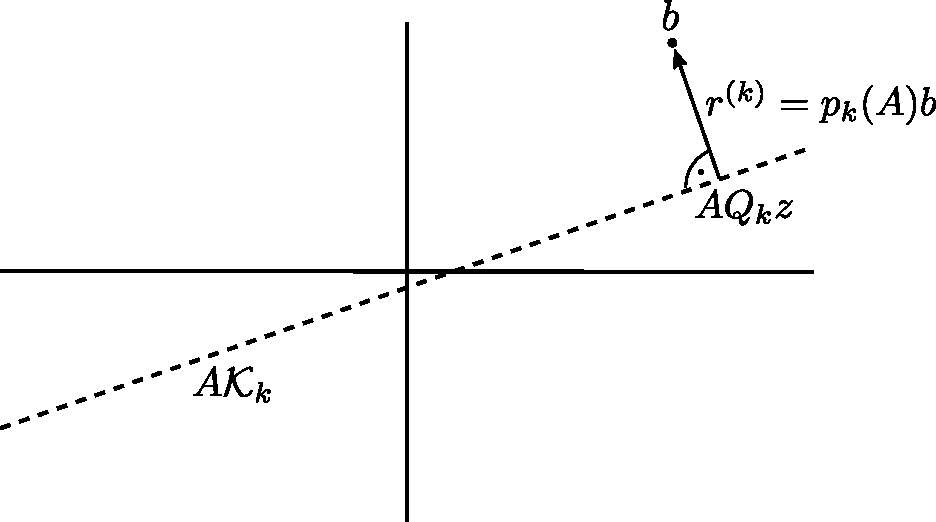
\includegraphics[width=0.7\linewidth]{figures/GMRES.pdf}
    \caption{The least squares polynomial approximation problem underlying the GMRES (minimizing $\norm{r_m}_2$), as described in \cite{trefethen_numerical_1997}}.
    \label{fig:gmres}
\end{figure}

\noindent It is evident that the column space of that matrix is $A\mathcal{K}_m$ and the problem is reduced to finding a vector $c \in \mathbb{R}^{m}$ such that $\norm{AK_mc-b}_2$ is minimal   \cite{trefethen_numerical_1997}. Once this vector is obtained, the approximate solution would be given by $x_m =K_mc$. Solving the least squares problem could be achieved by computing a QR factorization of $AK_m$, but this procedure would be numerically unstable, since $K_m$ is exceedingly ill-conditioned \cite{trefethen_numerical_1997}. Instead, Arnoldi's method is used to construct a sequence of Krylov matrices $Q_m$ (spanning the successive Krylov subspaces $\mathcal{K}_m$) and then setting the approximate solution to $x_m = Q_my$. Hence the problem can be reformulated as finding a vector $y \in \mathbb{R}^m$ satisfying:
\begin{equation}
    \norm{AQ_mz-b}_2=\text{ minimum}
\end{equation}

\noindent Using Equation~\hyperref[eqn:arnoldi]{\ref{eqn:arnoldi}} we obtain:
\begin{equation}
    \norm{Q_{m-1}\tilde{H}_m-b}_2=\text{ minimum}
\end{equation}

\noindent Now, multiplying by $Q^T_{m-1}$ from the left (which does not change the norm since both vectors are within the column space of $Q_{m-1}$), this is equivalent to:
\begin{equation}
    \norm{\tilde{H}_my-Q^T_{m-1}b}_2 = \text{ minimum}
\end{equation}

\noindent From the construction of the Krylov matrices $\{Q_m\}$ (Equations~\hyperref[eqn:krylov_space]{\ref{eqn:krylov_space}} \& \hyperref[eqn:krylov_matrix]{\ref{eqn:krylov_matrix}}) it follows that $q_1=b\:/\norm{b}_2$ and $q_i \perp b$, for $i = 2, \dots, m+1$. Therefore, $Q^T_{m+1}b$ is equal to $\norm{b}_2e_1$, where $e_1=(1,0,0,\dots)^T$ and the solution to the GMRES least squares problem can be obtained by:
\begin{equation}
    \norm{\tilde{H}_my-\norm{b}_2e_1}_2 = \text{ minimum}
\end{equation}

\noindent Due to the Hessenberg structure of $\tilde{H}_m$, this equation can be solved for $y$ via QR factorization at a reduced cost of $\mathcal{O}(m^2)$. Consequently GMRES is able to deliver a much faster solution than direct factorization, as long as the number of iterations $m$ remains small.

\begin{algorithm}[h]
  \caption{GMRES}
  \label{alg:gmres}
  \SetAlgoLined
  \DontPrintSemicolon
  \KwIn{non-singular matrix $A \in \mathbb{R}^{n \times n}$, vector $b \in \mathbb{R}^{n}$}
  \KwOut{approximate solution $x_m$ to the system $Ax=b$\\
  \hrulealg}
  $q_1= b\:/\norm{b}_2$ \\
  \% Arnoldi's method \\
  \For{$i = 1$ \KwTo $m$} {
    $w =A\cdot q^i$ \\
    \For{$j = 1$ \KwTo $i$} {
      $H_{j,i} = w^T\cdot q^j$ \\
      $ w = w - H_{j,i}\cdot q^j$}
    $H_{i-1,i} = \norm{w}_2$ \\
    \If{$H_{i-1,i} = 0$}{\Return $x_i$}
    $q^{i+1} = w/H_{i+1,i}$ \\
  }
  \;
  \% GMRES extension \\
  define $\tilde{H}_m = \{H_{i,j}\}, 1 \leq i \leq m+1, 1 \leq j \leq m$ \\
  define $Q_m = \{q_1, \cdots, q_m\}$ \\
  Find $y$ to minimize $\normd{\tilde{H}_my-\norm{b}_2e_1}_2$ ($=\norm{r_m}_2$) \\
  $x_m = Q_my$
\end{algorithm}

\noindent Algorithm~\hyperref[alg:gmres]{\ref{alg:gmres}} describes the general outline of the GMRES algorithm as provided by \cite{trefethen_numerical_1997} (based on Modified-Gram-Schmidt Arnoldi). From this, it is immediately evident that both storage and computational complexity are dependent on the number of iterations required. The original formulation of the algorithm \cite{saad_gmres_1986} differs slightly from the one given above, taking the residual as the starting vector for the iteration and solving the equation in line 18 for a correction term instead. This enables the method to be restarted from the current approximate solution after a certain number of iterations, preventing $m$ from growing prohibitively large. The required changes are illustrated in Algorithm~\hyperref[alg:gmres2]{\ref{alg:gmres2}}

\begin{algorithm}[h]
  \caption{GMRES (initial solution based)}
  \label{alg:gmres2}
  \SetAlgoLined
  \DontPrintSemicolon
  \KwIn{non-singular matrix $A \in \mathbb{R}^{n \times n}$, vector $b \in \mathbb{R}^{n}$, initial solution $x_0 \in \mathbb{R}^{n}$}
  \KwOut{approximate solution $x_m$ to the system $Ax=b$\\
  \hrulealg}
  $r_0 = b-Ax_0$ \\
  $\beta = \norm{r_0}_2$ \\
  $q1 = r_0/\beta$ \\
  \For{$i = 1$ \KwTo $m$} {
   $\langle$ step $i$ of Arnoldi's method (e.g. Algorithm~\hyperref[alg:arnoldi]{\ref{alg:arnoldi}} $\rangle$ \\
  }
  define $\tilde{H}_m = \{H_{i,j}\}, 1 \leq i \leq m+1, 1 \leq j \leq m$ \\
  define $Q_m = \{q_1, \cdots, q_m\}$ \\
  Find $y$ to minimize $\normd{\tilde{H}_my-\beta e_1}_2$ \\
  $x_m = x_0 + Q_my$
\end{algorithm}

A disadvantage of both variants of the algorithm is that they do not provide the approximate solution $x_m$ at each step and it is therefore difficult to determine how many iterations are needed. However, this issue can be alleviated by using plane rotations to transform the Hessenberg matrix into upper triangular form. Since this is a common technique for solving the problem $min(\normd{\tilde{H}_my-\beta e_1}_2)$, it can basically be performed at zero additional cost. By defining a sequence of rotations matrices $\Omega_i \in \mathbb{R}^{(m+1) \times (m+1)}$ of the form:
\begin{equation}
    \Omega_i=
    \begin{blockarray}{*{8}{c} l}
    \begin{block}{[*{8}{c}] l}
      1 & & & & & & & \\
      & \ddots & & & & & & \\
      & & 1 & & & & & \\
      & & &c_i & s_i& & &  \bigstrut[t] & \leftarrow \text{row } i\\
      & & &-s_i & c_i& & & \bigstrut[t] & \leftarrow \text{row } i+1\\
      & & & & & 1& & \\
      & & & & & & \ddots & \\
      & & & & & & & 1\\
    \end{block}
    \end{blockarray}
\end{equation}

\noindent Note that $s_i$ and $c_i$ are scalars satisfying $c^2_i+s^2_i=1$ and can generally be obtained via the formulas given in \cite{saad_iterative_2003}:
\begin{equation}
    s_i=\frac{H_{i+1, i}}{\sqrt{(H^{(i-1}_{i,i}=^2+H^2_{i+1, i}}}\text{,   } \;\;c_i=\frac{H^{(i-1)}_{i+1, i}}{\sqrt{(H^{(i-1}_{i,i}=^2+H^2_{i+1, i}}}
\end{equation}

\noindent By defining $V_m$ as the product of the rotation matrices $\Omega_i$
\begin{equation}
    V_m = \Omega_m \Omega_{m-1} \dots \Omega_1
\end{equation}
\noindent and
\begin{equation}
    \tilde{R}_m = V_m\tilde{H}_m 
\end{equation}
\begin{equation}
        \tilde{g}_m = V_m(\beta e_1) = (\gamma_1, \cdots, \gamma_{m+1})^T
\end{equation}

\noindent Thus, the problem can be reformulated as $min(\normd{\beta e_1 -\tilde{H}_my}_2==min(\normd{\tilde{g}_g -\tilde{R}_my}_2)$, thanks to $V_m$ being unitary. A detailed proof for this equation is given in \cite{saad_iterative_2003}. The big advantage of this method is not only that $\tilde{R}_m$ is triangular (and hence easily solvable), but also that the current residual (i.e. at step $m$) is readily available as $\gamma_{m+1}$.

Having obtained a satisfactory criterion to determine convergence, it is natural to ask for the upper bound of the number of iterations required by GMRES. Following the analysis in \cite{trefethen_numerical_1997}, we can observe that the algorithm converges monotonically, since $\norm{r_m}_2$ is minimal for the subspace $\mathcal{K}_m$, it can only decrease (or, at worst remain unchanged) by enlarging the space to $\mathcal{K}_{m+1}$.
\begin{equation}
    \norm{r_{m-1}}_2\leq \norm{r_m}_2
\end{equation}

\noindent Secondly, after at most $m$ steps, the process must converge in the absence of rounding errors and $\norm{r_m}_2 = 0$. However, to be useful as an iterative method, satisfactory accuracy must be achieved with  $m \ll n$. Expressed in terms of polynomial approximation: 
\begin{equation}
    \norm{r_m}_2=\norm{p_m(A)b}_2 \leq \norm{p_m(A)}_2\norm{b}_2
\end{equation}

\noindent And thus the convergence generally depends on the quantity $\norm{p_,(a)}_2$. This requires a polynomial that is as small as possible on the spectrum of $\Lambda(A)$, while still satisfying $p(0)=1$. For a diagonalizable matrix $A$, \cite{trefethen_numerical_1997} provide the following bound:
\begin{equation}
    \underset{p_m \in P_m}{\text{inf}} \norm{p_m(A)}_2 \leq \kappa(V) \underset{p_m \in P_m}{\text{inf}} \norm{p_m}_{\Lambda(A)}
\end{equation}

\noindent In this equation, $\Lambda(A)$ is the set of eigenvalues of $A$, $V$ is a non-singular matrix of eigenvectors, and $\norm{p_m}_{\Lambda(A)}$ is the smallest possible polynomial on the spectrum of $\Lambda(A)$ with $p(0)=1$. In other words, GMRES can only be expected to converge fast when $A$ is not too far from normal and properly normalized degree $m$ polynomials can be found whose size on the spectrum $\Lambda(A)$ decreases quickly. Hence the convergence does not only depend on the magnitude (i.e. conditioning) but also on the location of the eigenvalues of $A$.
As a closing statement with regards to the accuracy of the algorithm, it needs to be noted that \cite{paige_modified_2006} proved backward stability for the Modified-Gram-Schmidt variant of the algorithm. 